\section{Doli Jonviter NT Simbolon /1154016}
{\Large \textbf{Pemahaman Teori}}
\subsection{Soal 1}
Apa itu fungsi device manager di windows dan folder /dev di linux?

\hfill \break
Device Manager  dapat  membantu dalam mengelola  semua hardware yang terpasang  dalam suatu sistem Windows. 
 Berikut fungsi kegunaan Device Manager antara lain adalah :
\begin{enumerate}
	\item Menunjukkan status suatu hardware.
	\item Menunjukkan informasi detil suatu hardware.
	\item Mengelola driver hardware
	\item Disable dan Enable hardware
	\item Mengidentifikasi konflik antar perangkat keras.
\end{enumerate}

\hfill \break
Folder /bin merupakan isi program binner yang harus ada apabila sistem yang dipasang dalam mode single-user, dan juga  ada beberapa program penting seperti bash.

\subsection{Soal 2}
Jelaskan langkah-langkah instalasi driver dari arduino!

\hfill \break
Berikut ini adalah langkah-langkah instalasi driver dari Arduino UNO di Windows:

\begin{enumerate}
	\item Langkah pertama Hubungkan sistem minimun Arduino Uno ke komputer dengan kabel USB .
	\item Lalu pada bagian kanan didesktop PC , akan muncul popup “Installing device driver software” seperti pada gambar dibawah ini.
	\item Kemudian jika sistem  operasi Windows tidak menyediakan driver untuk Arduino Uno,maka harus  melakukan instalasinya harus dilakukan secara manual.
	\item Lalu  Buka Device Manager,  dengan cara pada bagian Search Program and Files lalu ketikkan “device manager” (tanpa tanda petik). 
	\item kemudian Pada bagian COntrol Panel akan muncul Device Manager, lalu klik untuk menjalankan program tersebut.
	\item Setelah itu cari  Unknown device pada bagian Other device, biasanya terdapat tanda seru berwarna kuning, itu disebabkan karena penginstallan gagal.
	\item Klik kanan pada bagian  “Unknown device” kemudian pilih Update Driver Software.
	\item kemudian cari Browse my computer for driver software pada laptop anda.
	\item setelah itu lakukan dengan mengklik Install pada tampilan Windows Security.
	\item Jika instalasi driver pada laptop anda berhasil maka akan muncul Windows has successfully updated your driver software.
	\item Perhatikan dan ingat nama COM Arduino Uno, karena nama COM ini yang akan digunakan untuk meng-upload program nantinya
\end{enumerate}

\subsection{Soal 3}
Jelaskan bagaimana cara membaca baudrate dan port dari komputer yang sudah terinstall driver!
\textbf{Membaca Baudrate dari Komputer}
\begin{enumerate}
	\item Pertama buka `Start'. Cari `Device Manager', lalu klik.
	\begin{figure}[H]
		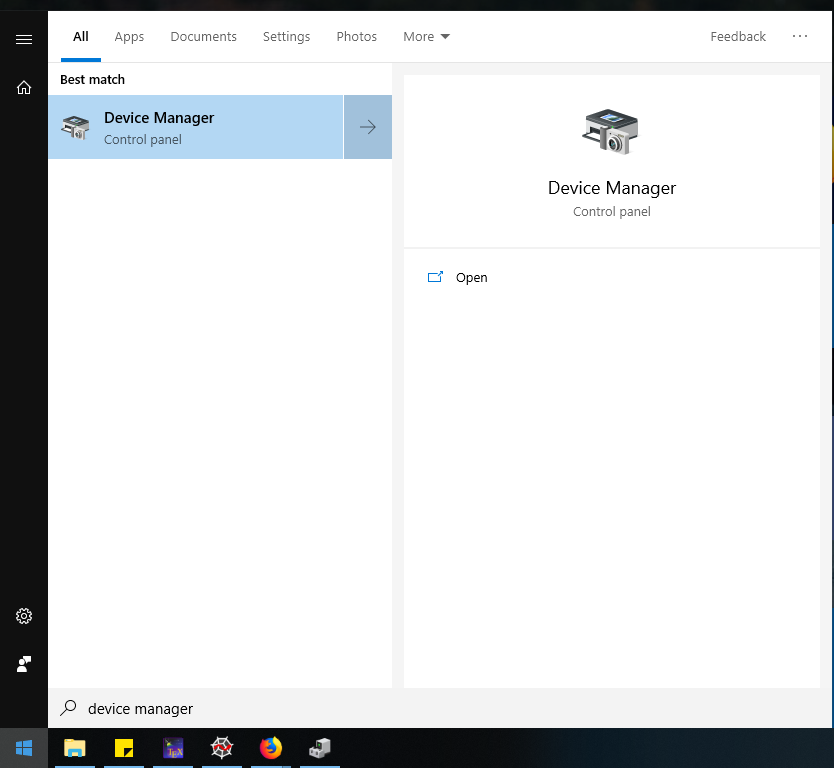
\includegraphics[width=5cm]{figures/5/1154016/Teori/d1.png}
		\centering
	\end{figure}
	\item Kemudian pilih `Ports (COM \& LPT)'.
	\begin{figure}[H]
		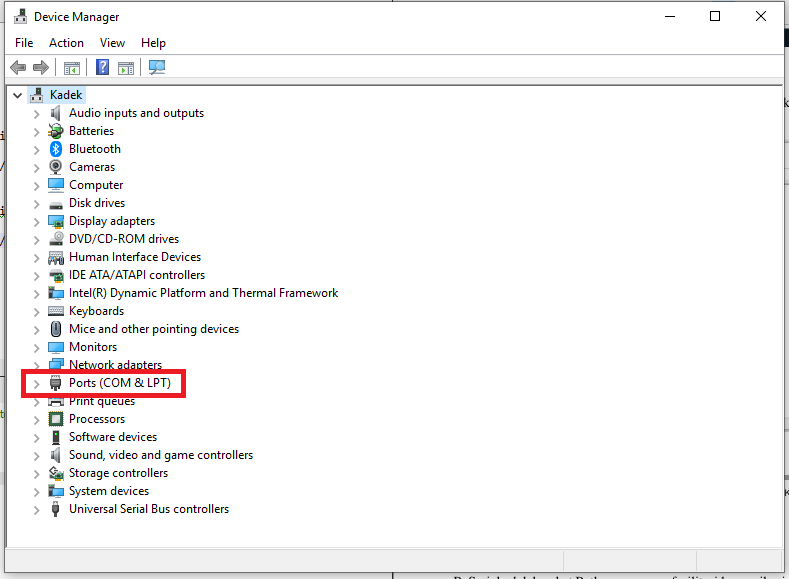
\includegraphics[width=5cm]{figures/5/1154016/Teori/d3.png}
		\centering
	\end{figure}
	\item Klik dua kali pada COM yang terhubung.
	\begin{figure}[H]
		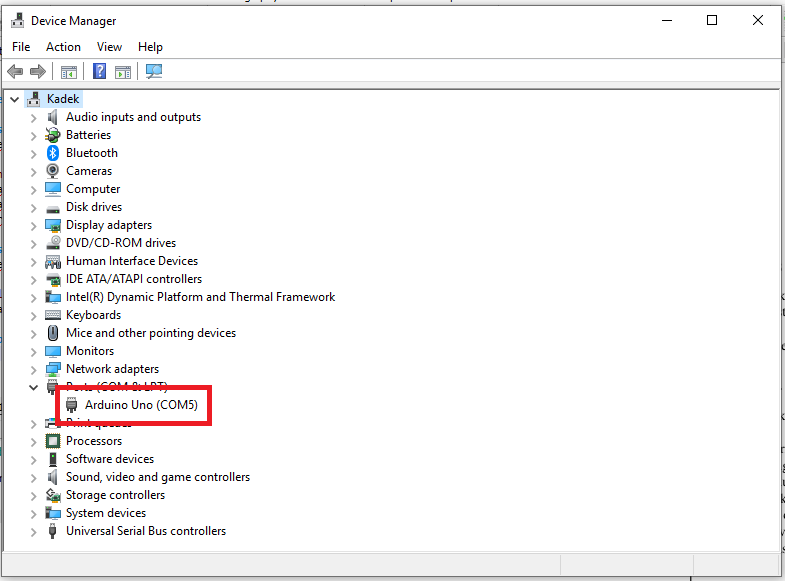
\includegraphics[width=5cm]{figures/5/1154016/Teori/d2.png}
		\centering
	\end{figure}
	\item Pilih tab `Port Settings', lalu lihat di `Bit per second'.
	\begin{figure}[H]
		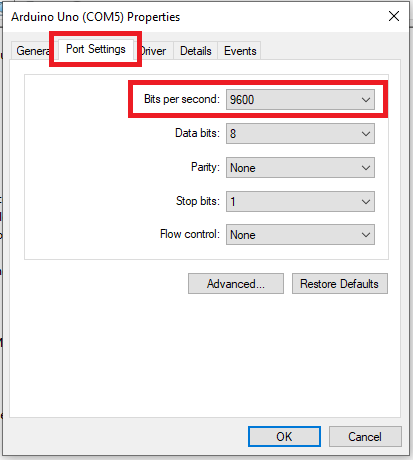
\includegraphics[width=5cm]{figures/5/1154016/Teori/d4.png}
		\centering
	\end{figure}
\end{enumerate}
\textbf{Membaca Port dari Komputer}
\begin{enumerate}
	\item Pertama buka `Start'. Cari `Device Manager', lalu klik.
	\begin{figure}[H]
		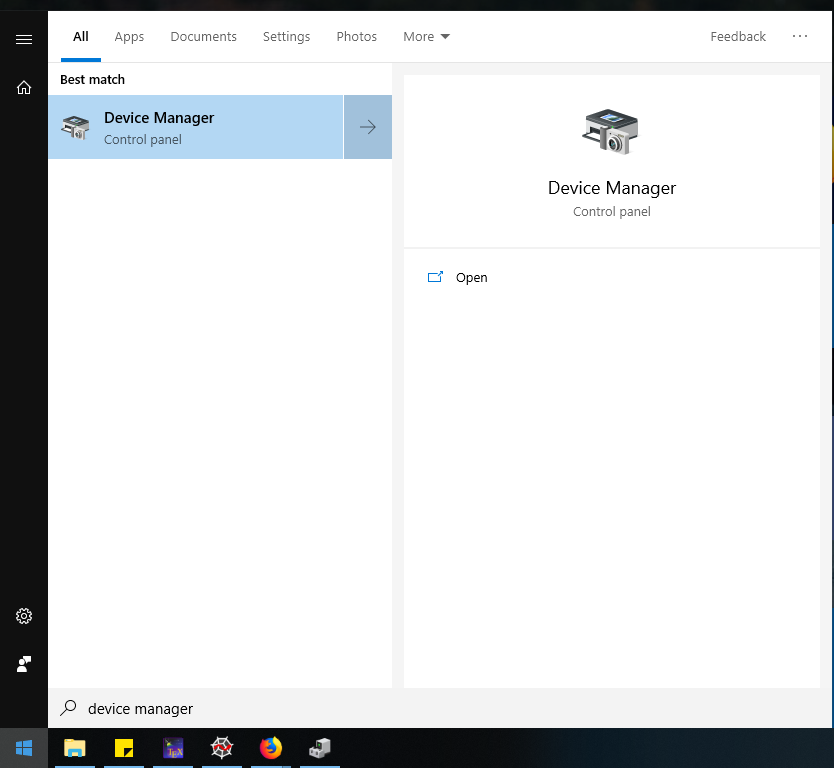
\includegraphics[width=5cm]{figures/5/1154016/Teori/d1.png}
		\centering
	\end{figure}
	\item Kemudian pilih `Ports (COM \& LPT)'.
	\begin{figure}[H]
		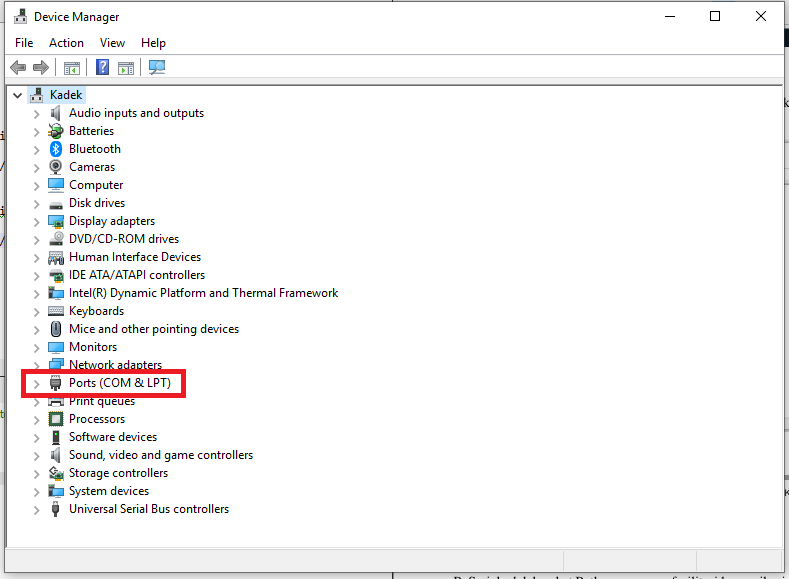
\includegraphics[width=5cm]{figures/5/1154016/Teori/d3.png}
		\centering
	\end{figure}
	\item Port dari Arduino telah terbaca oleh PC.
	\begin{figure}[H]
		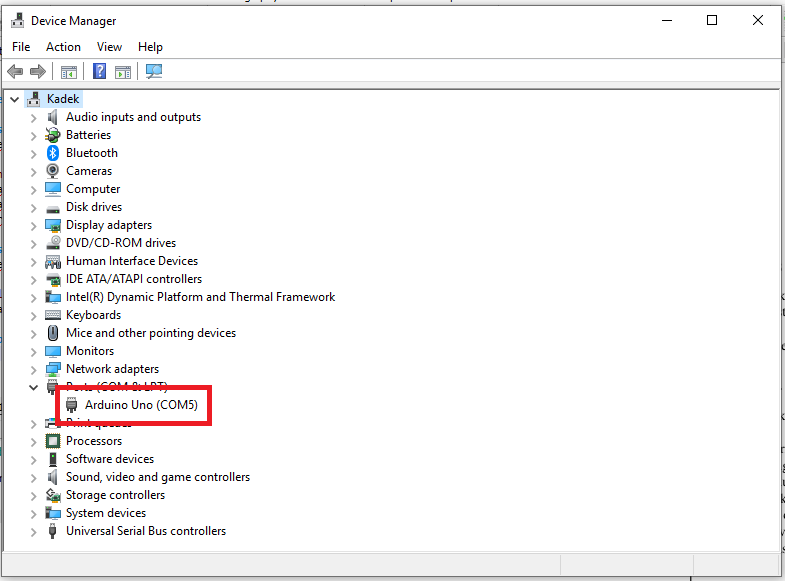
\includegraphics[width=5cm]{figures/5/1154016/Teori/d2.png}
		\centering
	\end{figure}
\end{enumerate}



\subsection{Soal 4}
Jelaskan sejarah library pyserial!.

\hfill \break
PySerial adalah paket Python yang memfasilitasi komunikasi serial antara PC dengan perangkat keras eksternal. PySerial menyediakan antarmuka untuk berkomunikasi melalui protokol komunikasi serial. Komunikasi serial adalah salah satu protokol komunikasi komputer tertua. Protokol komunikasi serial mendahului spesifikasi USB yang dapat digunakan oleh komputer dan perangkat keras lain seperti mouse, keyboard, dan webcam. USB adalah singkatan dari Universal Serial Bus. USB dibangun diatas dan memperluas antarmuka komunikasi serial asli.

\subsection{Soal 5}
Jelaskan fungsi-fungsi apa saja yang dipakai dari library pyserial!

\hfill \break
Fungsi-fungsi yang dipakai dari library PySerial, yaitu:
\begin{enumerate}
	\item Serial - fungsi ini untuk membuka port serial.
	\item write(data) - fungsi ini menulis data lewat port serial.
	\item readline() - fungsi ini membaca sebuah string dari port serial.
	\item read(size) - fungsi ini untuk membaca jumlah byte dari port serial.
	\item close() - fungsi ini untuk menutup port serial.
\end{enumerate}

\subsection{Soal No. 6}
Jelaskan kenapa butuh perulangan dan tidak butuh perulangan dalam membaca serial!

\hfill \break
Pada saat membaca serial di Arduino diperlukan perulangan agar dapat membaca data secara berulang kali sehingga data yang muncul banyak. Sedangkan apabila tidak membutuhkan perulangan maka Arduino hanya akan membaca data sekali saja.

\subsection{Soal No. 7}
Jelaskan bagaimana cara membuat fungsi yang mengunakan pyserial!

\hfill \break
Fungsi yang berada pada Python, dibuat dengan nama kata kunci def kemudian diikuti dengan nama fungsinya pada pyhton.
Seperti halnya dengan blok kode yang lain, kita juga harus memberikan identasi untuk menuliskan isi fungsi.
